\newcommand{\argmin}{\mathop{\mathrm{arg\,min}}}
\newcommand{\norm}[1]{\left\lVert#1\right\rVert}
% This thesis template is based on the report class of
% latex. Yout do not need to change this.
\documentclass[12pt, a4paper]{report}
\usepackage{amsmath}
\usepackage{subfig}
\usepackage{hyperref}
% This includes all variables that are used in this work
% Use this document to specify your name, your reviewers
% and other values that you would like to maintain
% in one place.
\newcommand\myname{Julian Bialas, BSc}
\newcommand\mypkz{1910837917}

\newcommand\myfirstreviewer{Prof. (FH) PD Dr. Mario Döller}
% Leave second review empty for bachelor's thesis
\newcommand\mysecondreviewer{Sebastian Danninger, MA}

\newcommand\mytitle{Autonomous Modeling of a 3D Environment with Drones}

% The value below is the date that you finished your work. This
% date appears on you work's cover page and in the "Eidesstattliche
% Erklärung".
\newcommand\mydate{18. Juni 2021}

% For a master's thesis use MA as type, BA for a bachelor's thesis
\newcommand\type{MA}

% Set the name of your study program. 
% DSIA for Data Science & Intelligent Analytics
% WEB for Web Business & Technology
% WCIS for Web Communications and Information Systems
% SPS for Smart Products and Solutions
\newcommand\program{DSIA}

% Define the language in which you write this thesis
% Use DE for German, EN for English
\newcommand\lang{EN}


% This includes all packages and presets. You do not need
% to change this file unless you want to add new packages
% or change the presets of one of the used packages.
%\usepackage{bookman}  % Font package
%\usepackage[light]{CrimsonPro}
\usepackage{pxfonts}
\usepackage[T1]{fontenc}
\usepackage{graphicx}
\usepackage[utf8]{inputenc}
\usepackage{blindtext}  % Used for dummy text segments
\usepackage{natbib}
\usepackage{hyperref}
\usepackage{booktabs}
\usepackage{xcolor}
\usepackage{listings}
\lstset{numberbychapter=false}
\iflanguage{english}{\renewcommand{\lstlistlistingname}{List of Listings}}{\renewcommand{\lstlistlistingname}{Listingsverzeichnis}}

\usepackage{fancyhdr}  % Head and footer styling
\fancyhf{}
\fancyhead{}
\fancyfoot[CO]{\thepage}
\renewcommand{\headrulewidth}{0pt}
\renewcommand{\footrulewidth}{0pt}


\usepackage[a4paper, left=3.5cm, right=3cm, top=3.5cm, bottom=3cm]{geometry}
\setlength{\headheight}{15pt}


\usepackage{titlesec}
\titleformat{\chapter}{\bf \LARGE}{\thechapter.}{16pt}{\LARGE}

\bibliographystyle{apalike}
\pagestyle{headings}
\setlength{\parindent}{0em}
\setlength{\parskip}{1.5em}
\renewcommand{\baselinestretch}{1.13}  

\lstset{
    numberstyle=\tiny,
    numbers=left,
    showstringspaces=false,
    breaklines=true,
    commentstyle=\itshape\color{darkgray},
    basicstyle=\ttfamily,
    stringstyle=\color{orange},
    keywordstyle=\bf\color{green!40!black},
    identifierstyle=\color{blue}
}

\hypersetup{
  pdftitle    = \mytitle,
  pdfsubject  = \worktype,
  pdfauthor   = \myname,
  pdfcreator  = {pdflatex using template provided by University of Applied Sciences FH Kufstein Tirol},
  bookmarksnumbered = true,
  colorlinks = true,
  linkcolor = blue,
  citecolor = green,
  urlcolor = orange
}


% This includes custom latex commands. You can use this
% file to create your own command sequences.
\newcommand{\fh}{\textsc{FH Kufstein Tirol}}

\newcommand{\fig}[4]{
    \begin{figure}[ht]
        \centering
        \includegraphics[width=#4\textwidth]{#1}
        \caption{#2}
        \label{#3}
    \end{figure}
}


% If you want to print your thesis in black and white
% uncomment the following section

% \hypersetup{
%     colorlinks=false,
%     pdfborder = 0 0 0
% }
% \lstset{
%     commentstyle=\itshape,
%     basicstyle=\ttfamily,
%     stringstyle=\color{black},
%     keywordstyle=\bf,
%     identifierstyle=\color{black}
% }

\begin{document}

    \frontmatter

    % This places the front matter. You do not need to 
    % change this file. All thesis-specific values are 
    % imported from "variables.tex".
    \begin{titlepage}
 
    \vfill
    \begin{center}
      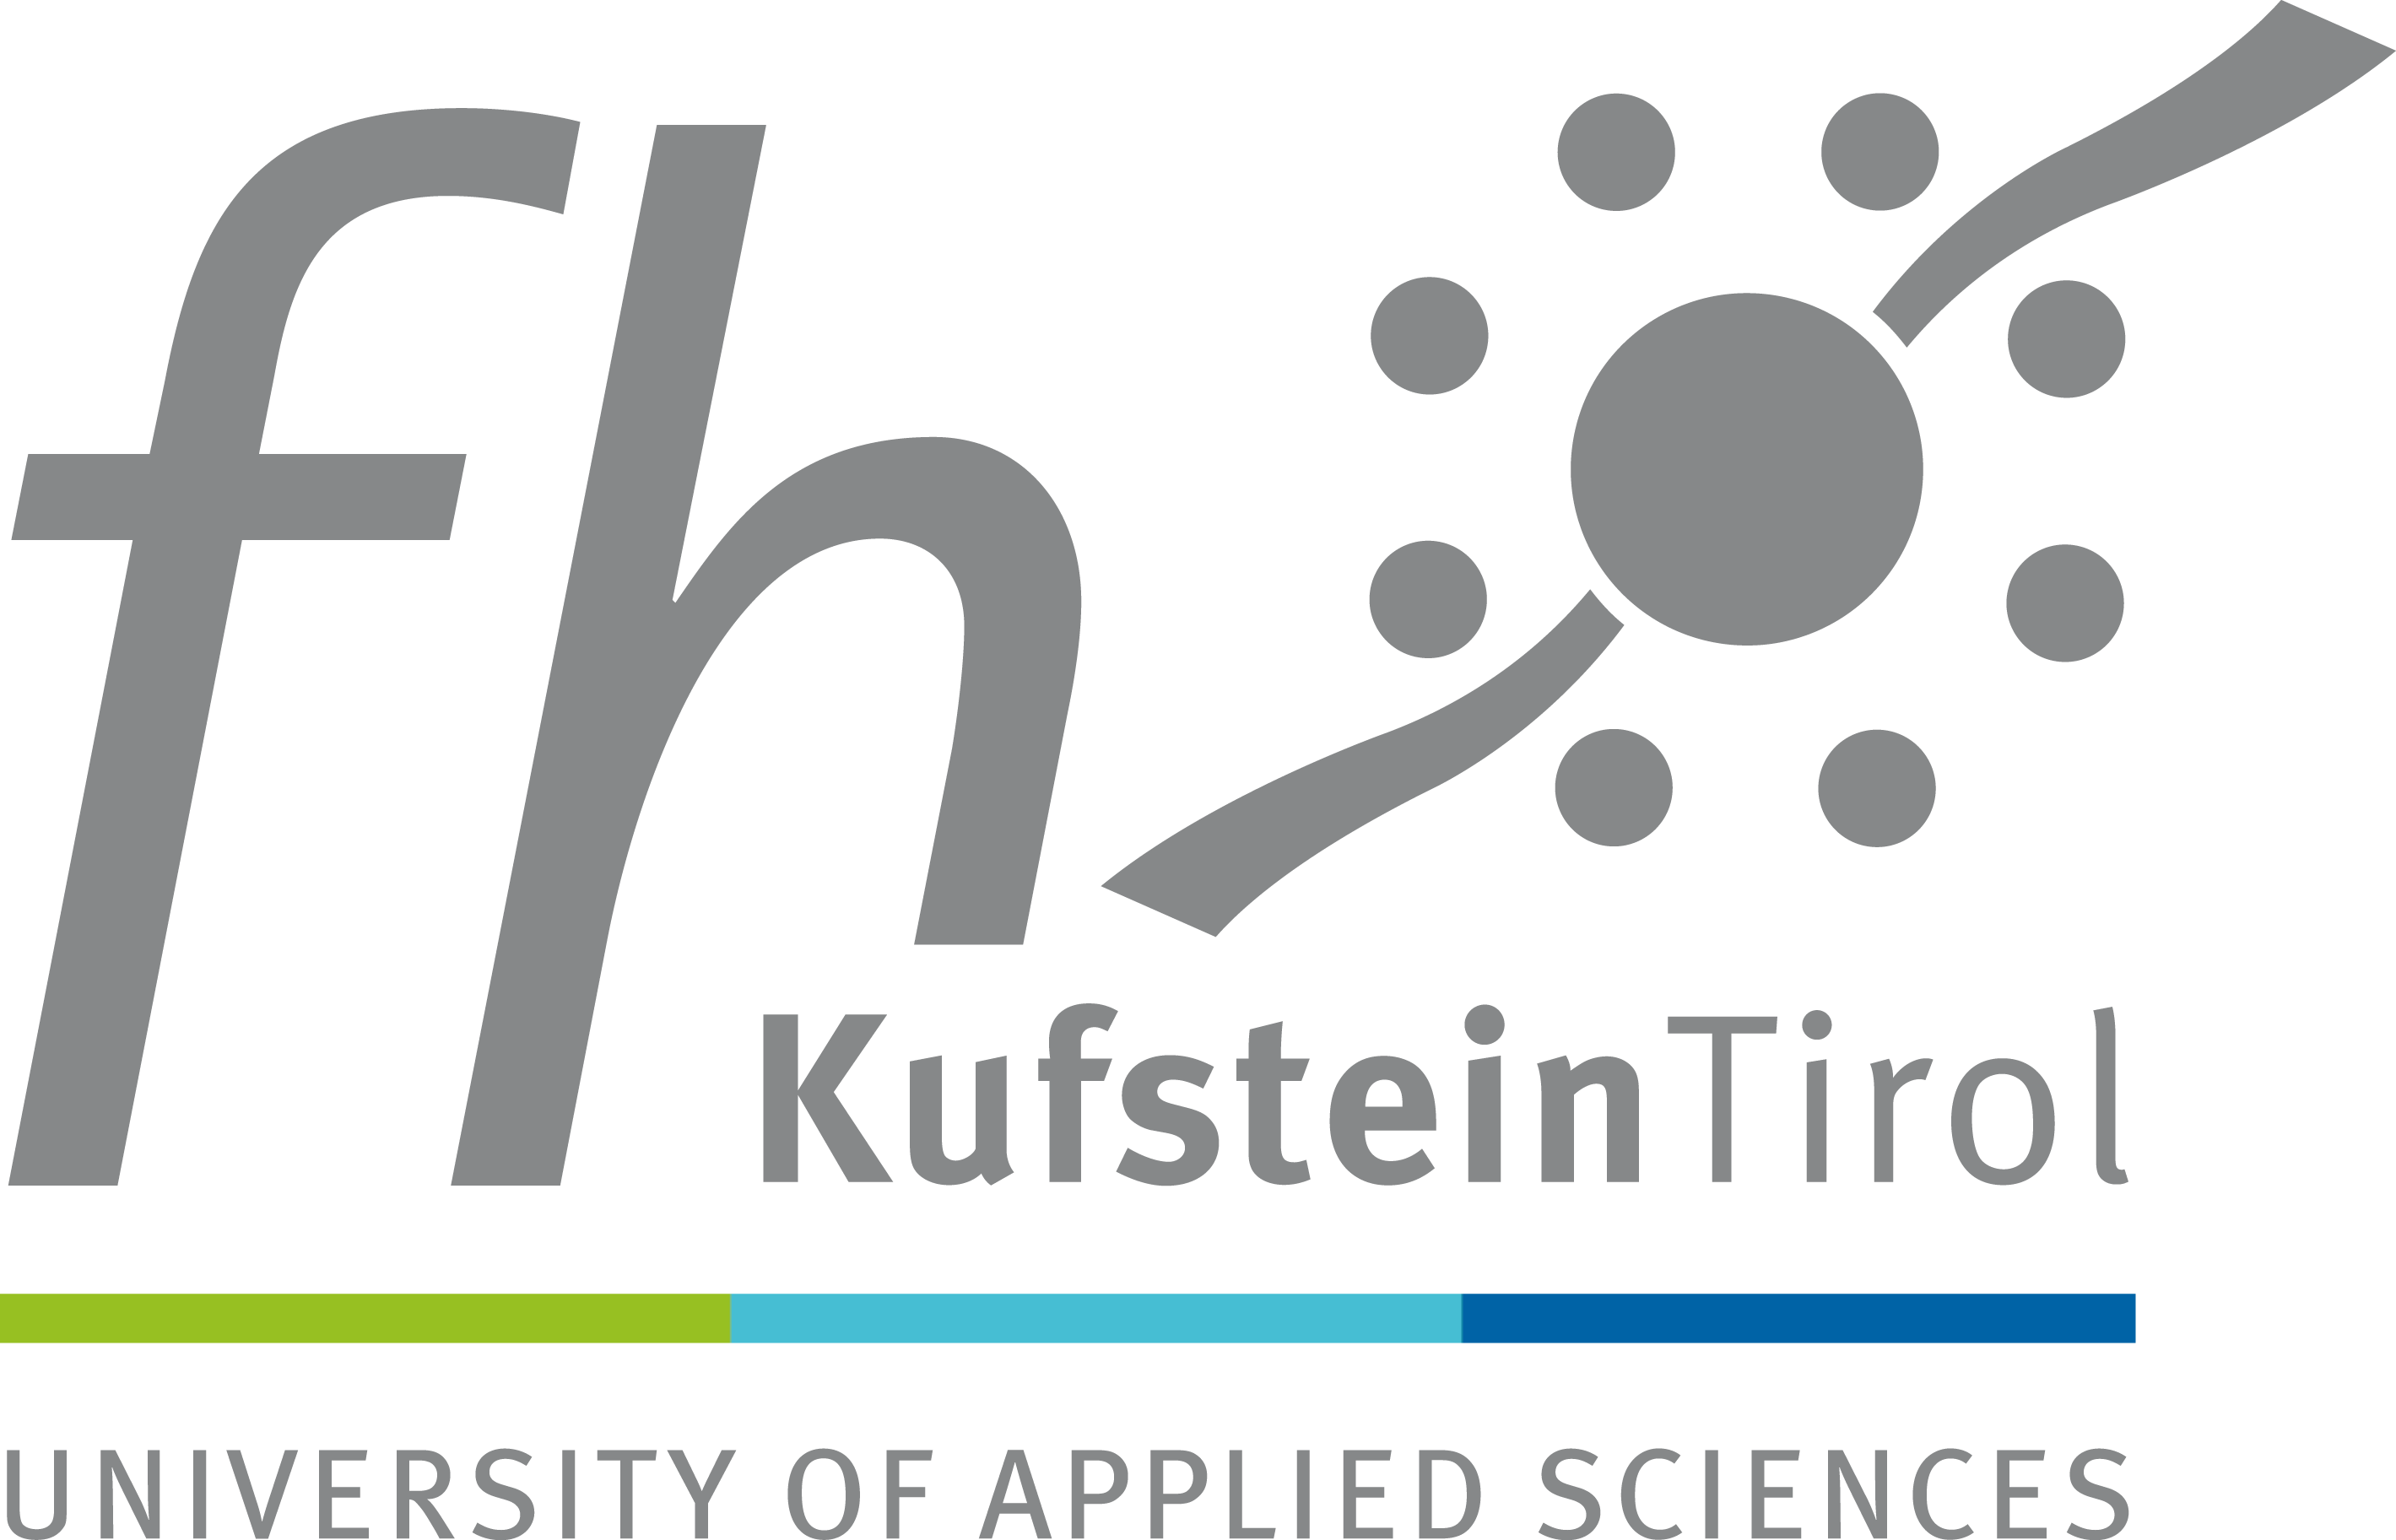
\includegraphics[width=4.5cm]{img/kufstein_logo.png} \\ 
    \end{center}
    \vfill
  
    \begin{center}
      \Large \textbf{\mytitle}
    \end{center} 
    \vfill
  
    \begin{center}
      %\condMASTER{\Large Masterarbeit}{\Large Bachelorarbeit}
      \worktype
    \end{center}
    \vfill
  
    \begin{center}
      zur Erlangung des akademischen Grades\\
      \large \textbf{\academictitle}
    \end{center}
    \vfill
  
    \begin{center}
      Eingereicht bei:\\ 
      \vspace{0.1cm}
      \large \textbf{Fachhochschule Kufstein Tirol Bildungs GmbH}\\
      \vspace{0.1cm}
      \large \textbf{\studyprogram}
    \end{center}
    \vfill
  
    \begin{center}
      Verfasser/in:\\
      \vspace{0.1cm}
      \large \textbf{\myname}\\
      \vspace{0.1cm}
      \large \textbf{\mypkz}\\
    \end{center}
    \vfill
  
    \begin{center}
      \begin{tabular}{lll}
        \ifthenelse{\equal{\type}{MA}}{
          Erstgutachter  & : & \myfirstreviewer \\
          Zweitgutachter & : & \mysecondreviewer
        }{
          Gutachter  & : & \myfirstreviewer \\
        }
      \end{tabular}
    \end{center} 
    \vfill
  
    \begin{center}
      Abgabedatum: \\
      \vspace{0.1cm}
      \large \textbf{\mydate}
    \end{center} 
    \vfill  
  \end{titlepage}


    % This places the "Eidesstattliche Erklärung". This 
    % Document is always in German, even if your work is
    % written in English.
    \chapter*{Eidesstattliche Erklärung}
\thispagestyle{empty}

Ich erkläre hiermit, dass ich die vorliegende \worktype selbständig und ohne fremde Hilfe verfasst und in der Bearbeitung und Abfassung keine anderen als die angegebenen Quellen oder Hilfsmittel benutzt sowie wörtliche und sinngemäße Zitate als solche gekennzeichnet habe. Die vorliegende \worktype wurde noch nicht anderweitig für Prüfungszwecke vorgelegt.

\vspace{2cm}
Kufstein, \mydate

\vspace{2cm}
\rule{10cm}{1pt}\\
\myname{}



    % This will include a "Sperrvermerk". This document
    % is always in German, even if your work is written
    % in English. Please remove this line, if necessary.
    \chapter*{Sperrvermerk}
\thispagestyle{empty}

Ich habe die Sperrung meiner \worktype beantragt, welche von der Studiengangsleitung genehmigt wurde.

\vspace{2cm}
Kufstein, \mydate

\vspace{2cm}
\rule{10cm}{1pt}\\
\myname{}


    % This inserts all necessary tables into your work.
    \tableofcontents
    \listoffigures
    \listoftables

    % Use this if you have any code listings
    \lstlistoflistings

    % Use this if you want to use acronyms
    \acro{html}[HTML]{HyperText Markup Language}
\acro{js}[JS]{JavaScript}


    \markboth{}{}

    % This adds a german and an english summary to your work.
    % You always have to add both, independent of whether your
    % work is done in german or english
    % Your text goes here (aprox. 350 words)
\Blindtext[2][1]

    % Your text goes here (aprox. 350 words)
\Blindtext[2][1]


    \mainmatter

    % This places the actual chapters. The files referenced here
    % are just an example. You can add additional chapters if 
    % necessary
    \chapter{Introduction}

Multiple applications exist for the autonomous exploration and mapping tasks using drones,
 such as search and rescue-, inspection- and surveillance operations \cite{usecases}. 
 
 The autonomous exploration task can be divided into three subproblems: localization, mapping, and path planning \cite{accurat}. 
 All three tasks should be performed simultaneously within an environment, which the drone has no information on a priori. 
 
 The localization task contains the estimation of the position of the drone within this environment and the mapping task refers to 
 the incremental creation of a 3-dimensional map. There are several methods that combine these two tasks in a so-called 
 simultaneous localization and mapping (SLAM) algorithm. The development of these SLAM algorithms is one of the most researched topics 
in the field of robotics \cite{slamintro}.

\begin{quote}
SLAM is used for many applications including mobile robotics, self-driving cars, unmanned
aerial vehicles, or autonomous underwater vehicles \cite{quote1}.
\end{quote}

 When combining a SLAM algorithm with a path planning algorithm, an autonomous exploration 
system is created. The autonomous exploration using SLAM and a path planning algorithm is sometimes also referred to as active SLAM \cite{inproceedings}. 
This active SLAM process is displayed in figure \ref{fig:autsys}. Details on how such a system can be initiated and terminated, can be found in section 
\ref{rosframe}.
 
 \fig{img/aut_system.png}{Automated exploration system, based on a SLAM algorithm and a path planning algorithm. }{fig:autsys}{0.9}
 
This work targets to answer two distinct research questions. 
 
 \begin{enumerate}
 \item{What is the most suitable open-source monocular visual SLAM algorithm for an exploration task?}
 
 
  This work is limited to evaluate monocular visual SLAM (vSLAM) algorithms, meaning that the algorithm is only working
 with a single RGB (red, green, blue) camera as sensor. Therefore, since nowadays RGB cameras are either a standard on drones or can easily be upgraded,
 these drones are very affordable, making it highly available for a larger user group. 
 
 
 Thus, in the first part of this work, three open-source monocular visual SLAM algorithms are evaluated. 
  DSO (Direct Sparse Odometry) SLAM, DSM (Direct Sparce Mapping) SLAM and ORB (Oriented FAST and Rotated BRIEF)
 SLAM were investigated regarding the predefined criteria of the accuracy of the resulting trajectory estimation, the point cloud accuracy and computational speed. 
 
 This was done by using the publicly available benchmark EuRoC dataset \cite{euroc}, containing video sequences filmed by a drone, the 
 ground truth of the position of the drone and the point cloud of the environment. Thus, the three SLAM algorithms are applied on the 
 video sequences, the resulting trajectories and map points are compared to the ground truth regarding the above-mentioned criteria.

 \item{What is a suitable framework to test and develop fully automated exploration systems within a simulated environment?}
 
 
 In the second part of this work, a Roboter Operating System (ROS) framework that enables users to develop a fully automated exploration system within 
 a virtual environment is proposed. This framework includes a process that provides a simulated Gazebo environment, making it possible to navigate 
 a virtual drone within a simulated environment. The sensors and behavior of the drone are modeled realistically. Most importantly, the drone is equipped with a RGB 
 camera, which allows the direct application of a vSLAM algorithm on the output. 
 Furthermore, the most suitable algorithm, evaluated in the first part of the work is implemented in a subprocess of this framework. 
 
 While the functionality and current state of the art of methods tackling the path planning task of the automated system are described and a suggestion on how it could 
 be implemented into the framework is given in section \ref{path}, this work does not include an actual implementation of such an algorithm. 
 Such implementations are left for further research. 
 
 The suggested framework should rather function as an option for users to implement and test out new path planning algorithm, providing optimal 
 prerequisites to do so. 
 
 For example, the subprocess of the framework, in which the path planning algorithm should run can be provided with all necessary data, 
 such as sensor data of the drone and the estimated orientation, position and point cloud by the vSLAM algorithm. This stream data is preprocessed 
 and standardized 
 in real time, enabling users to directly use it for their purposes. 
 
 
\end{enumerate} 
 
 





    \chapter{Methods}
\section{vSLAM Algorithms}
% hier erklrung von direct and feature methods
	\subsection{ORB-SLAM}
	
	ORB SLAM is a feature based, state of the art slam method. The first version was published in 2015 \cite{orb}. 
	Here, an overview of the functionality of ORB SLAM is provided. The Algorithms runs on three threats simultanously.
	Each thread performes one of the following tasks: Tracking, Local Mapping and Loop Closing. An overview over the tasks can be found 
	in figure \ref{fig:orb_fig}. The explaination of these system components are described in the following subsections.
	
	\fig{img/orb_slam_overview.png}{Overview of the system components extracted from \cite{orb}}{fig:orb_fig}{0.6}
	
	\subsubsection{Tracking}
	
	The tracking component determines the localization of the camera and decides, when a new keyframe is beeing inserted. 
	
	% keyframe noch beschreiben. 
	
	First, feature matching with the previous frame is performed, then the pose is optimized using motion only bundle adjustment. 
	
	% ? feature matching, bundle adjustment
	
	
	

	

	\subsection{DSM-SLAM}

	\subsection{DSO-SLAM}
	

\section{Calculations}

	\subsection{Trajectory Alignment}
	
	In order to compare the evaluated position of the camera at a given time with the ground truth of the 
	position, the trajectories need to be aligned. This is because most SLAM Algorithms innitilize the origin
	of their coordinate system with the camera position from the first frame. Whereas the ground truth of the 
	trajectory uses a different origin. As a consequence, evaluated points $ \left\{{\widehat{p}_i}\right\}_{i=0}^{N-1} $ can not be 
	compared to the ground truth points $ \left\{{p_i}\right\}_{i=0}^{N-1} $
	Also, as described in the vSLAM Algorithms section,
	
	% input link of section here
	
	the minority of the existing vSLAM algorithms are recognizing the true scale of the coordinate system. For
	those two reasons, the target is to find $S = \left\{R,t,s\right\}$, while $R$ being a rotation matrix, $t$ a translation vector
	and $s$ a scaling factor, 
	such that
	
	$$ S = \argmin_{S' = \left\{R', t', s' \right\}} \sum_{i = 0}^{N-1} \norm{p_i - s'R'\widehat{p}_i - t'}^2 $$ .
	
	In other words, the evaluated points are rotated, translated and scaled in a way, that the sum squared error over the point
	distances is minimized. The upper expresssion is calculated by using the method of Umeyama \cite{ume}. 
	
	Similar to principal component analysis, Umeyama uses the singular value decomposition of the covarianve 
	matrix $\Sigma$ of $p$ and $\widehat{p}$. Thus, 
	$\Sigma = UDV^T$ is yielded. Umeyama proves, that $R,t$ and $s$ can be calculated as followed: 
	
	$$ R = UWV^T $$
	$$ s = \frac{1}{\sigma^2_p}\text{tr}\left(DW\right)$$
	$$ t = \mu_{\widehat{p}} - sR\mu_p $$
	
	with 
	
	$$ W = \begin{cases}
      I, & \text{if}\ \text{det}\left(U\right)\text{det}\left(V\right) =0 \\
      \text{diag}\left(1,1,-1\right), & \text{otherwise}
    \end{cases}$$
	$\sigma_p$ beeing the standard deviation of $p$, $\mu$ the mean and $\text{tr}$ the trace of a matrix. 
	

\section{Datasets}

	\subsection{EuRoC Dataset}

	For the evaluation of the vSLAM Algorithms, the EuRoC dataset \cite{euroc} was used.
	The dataset contains eleven video sequences, recorded with a micro aerial vehicle at 20 frames per second.
	The sequences have a resultion of 752x480 pixels.
	For each Sequence, RGB images from two cameras exist. However, since the evaluation
	focuses on monocular SLAM methods, only the left camera was considered. Also the available 
	inertial and camera pose data was not taken in consideration. The first five sequences were recorded in 
	the machine hall at ETH Zürich, and the other six were recorded in a room, that was provided 
	with additional obsticals. For the latter six sequences, the groundtruth of the environment 
	exists as a dense pointcloud, as can be seen in figure \ref{fig:pcgt}.

	\fig{img/pointcloud_gt.png}{Pointcloud ground truth of sequence V1\_01\_easy visualized with python package pptk}{fig:pcgt}{0.7}

	Finally the true position of the 
	camera is known at a high frequency of over 200 points per second. 
	An overview of the sequences is shown in table \ref{table:euroctable}.



	\begin{table}
	\caption{Overview of the sequences included in the EuRoC Dataset}
	\begin{tabular}{ |p{3cm}||p{3cm}|p{3cm}|p{3cm}|  }
	\hline
	Sequence Name& Duration in $s$ & Average Velocity in $ms^{-1}$ &Pointcloud available\\
	\hline
	MH\_01\_easy & 182 & 0.44 & No\\
	MH\_02\_easy & 150 & 0.49 & No\\
	MH\_03\_medium & 132 & 0.99 & No\\
	MH\_04\_difficult & 99 & 0.93 & No\\
	MH\_05\_difficult & 111 & 0.88 & No\\
	V1\_01\_easy & 144 & 0.41 & Yes\\
	V1\_02\_medium & 83.5 & 0.91 & Yes\\
	V1\_03\_difficult & 105 & 0.75 & Yes\\
	V2\_01\_easy & 112 & 0.33 & Yes\\
	V2\_02\_medium & 115 & 0.72 & Yes\\
	V2\_03\_difficult & 115 & 0.75 & Yes\\
	\hline
	\end{tabular}
	\label{table:euroctable}
	\end{table}
	
\section{Setup and Environment}

	\subsection{Evaluation}
	
	The entire evaluation is run on a virtual machine. The host system is a lenovo yoga with eight GB of RAM and the basic model (8250U CPU @1.6 
	GHz 1.80GHz) of an eight core i5. The operating system of the host machine is Windows 10 Home. The virtual
	machine is given 5 GB of Ram and 4 cores. The operating system of the virtual machine is Ubuntu 18.04. All further setup information can be extracted 
	from the github repository.

	\subsection{Flight Path Planning}
 
 
	\section{Evaluation Methods}\label{methsec}

To evaluate the performance of DSO-, DSM- and ORB-SLAM, the algorithms are fed with video sequences contained in the 
European Robotics Challenge (EuRoC) benchmark dataset. The algorithms are changed in a way, that they save the computed 
trajectory estimation to a .txt file and the resulting point cloud to a .PLY file. 

Because an algorithm run on the same sequence can yield different results, each sequence is fed three times to the algorithm. 
This way, the results are more reproducible. 

\subsection{Dataset}

	For the evaluation of the vSLAM Algorithms, the EuRoC dataset \cite{euroc} was used.
	The dataset contains eleven video sequences, recorded with a micro aerial vehicle at 20 frames per second.
	The sequences have an image resolution of 752x480 pixels.
	
	For each Sequence, RGB images from two cameras exist. However, since the evaluation
	focuses on monocular SLAM methods, only the left camera was considered. Also the available 
	inertial and camera pose data was not taken in consideration. 
	
	The first five sequences were recorded in 
	the machine hall of the Eidgenössische Technische Hochschule Zürich, and the other six were recorded in a room, that was provided 
	with additional obstacle. For the latter six sequences, the ground truth of the environment 
	exists as a dense point cloud, as can be seen in figure \ref{fig:pcgt}.

	\fig{img/pointcloud_gt.png}{Point cloud ground truth of sequence V1\_01\_easy visualized with python package pptk}{fig:pcgt}{0.9}

	Finally the true camera pose $\in \text{SE}(3)$ of the 
	camera is known at a high frequency of over 200 points per second. This includes the camera position and the camera orientation. 
	
	An overview of the sequences is shown in table \ref{table:euroctable}. For each sequence, the average camera velocity, rotation velocity duration 
	are given. 



	\begin{table}
	\caption{Overview of the sequences included in the EuRoC Dataset}
	\begin{tabular}{ |p{3cm}||p{3cm}|p{3cm}|p{3cm}|}
	\hline
	Sequence Name& Duration in $s$ & Average Velocity in $ms^{-1}$ &Point cloud available\\
	\hline
	MH\_01\_easy & 182 & 0.44 & No\\
	MH\_02\_easy & 150 & 0.49 & No\\
	MH\_03\_medium & 132 & 0.99 & No\\
	MH\_04\_difficult & 99 & 0.93 & No\\
	MH\_05\_difficult & 111 & 0.88 & No\\
	V1\_01\_easy & 144 & 0.41 & Yes\\
	V1\_02\_medium & 83.5 & 0.91 & Yes\\
	V1\_03\_difficult & 105 & 0.75 & Yes\\
	V2\_01\_easy & 112 & 0.33 & Yes\\
	V2\_02\_medium & 115 & 0.72 & Yes\\
	V2\_03\_difficult & 115 & 0.75 & Yes\\
	\hline
	\end{tabular}
	\label{table:euroctable}
	\end{table}

\subsection{Evaluation Criteria}
\subsubsection{Trajectory Comparison}

	\begin{enumerate}
	\item{Trajectory Alignment}
	
	In order to compare the evaluated position of the camera at a given time with the ground truth of the 
	position, the trajectories need to be aligned. This is because most SLAM Algorithms initialize the origin
	of their coordinate system with the camera position from the first frame. Whereas the ground truth of the 
	trajectory uses a different origin and orientation. As a consequence, evaluated points $ \left\{{\widehat{x}_i}\right\}_{i=0}^{N-1}$ can not be 
	compared to the ground truth points $\left\{{x_i}\right\}_{i=0}^{N-1}$
	Also, as described in the vSLAM Algorithms section,
	
	% input link of section here
	
	the minority of the existing vSLAM algorithms are recognizing the true scale of the coordinate system. For
	those two reasons, the target is to find $S = \left\{R,t,s\right\}$, while $R$ being a rotation matrix, $t$ a translation vector
	and $s$ a scaling factor, 
	such that
	
	$$ S = \argmin_{S' = \left\{R', t', s' \right\}} \sum_{i = 0}^{N-1} \norm{x_i - s'R'\widehat{x}_i - t'}^2 $$ .
	
	In other words, the evaluated points are rotated, translated and scaled in a way, that the sum squared error over the respective point
	distances is minimized. The upper expression is calculated by using the method of Umeyama \cite{ume}. 
	
	Similar to principal component analysis, Umeyama uses the singular value decomposition of the covariance 
	matrix $\Sigma$ of $x$ and $\widehat{x}$. Thus, 
	$\Sigma = UDV^T$ is yielded. Umeyama proves, that $R,t$ and $s$ can be calculated as followed: 
	
	$$ R = UWV^T $$
	$$ s = \frac{1}{\sigma^2_p}\text{tr}\left(DW\right)$$
	$$ t = \mu_{\widehat{x}} - sR\mu_p $$
	
	with 
	
	$$ W = \begin{cases}
      I, & \text{if}\ \text{det}\left(U\right)\text{det}\left(V\right) =0 \\
      \text{diag}\left(1,1,-1\right), & \text{otherwise}
    \end{cases}$$
	$\sigma_p$ being the standard deviation of $x$, $\mu$ the mean and $\text{tr}$ the trace of a matrix. 
	
	\item{Positional Error}
	
	The error between $\left\{{\widehat{x}_i}\right\}_{i=0}^{N-1}$ and $\left\{{x_i}\right\}_{i=0}^{N-1}$ is computed after aligning them 
	with the upper method using the computed parameters $S = \left\{R,t,s\right\}$, yielding
	
	$$ \widehat{x}_i' = sR\widehat{x}_i - t $$
	
	. Then the distances between the points are evaluated using the euclidean norm: 
	
	$$ e_i = \lVert \mathbf{\widehat{x}_i' - x_i} \rVert_2$$
	
	\fig{img/trajectory_error.png}{Trajectory error after alignment. Source: \cite{tutorial}}{fig:trerror}{0.8}
	
	In figure \ref{fig:trerror} the computed errors are displayed. 
	
	
	These error terms are visualized over time and the overall mean is determined and again visualized with boxplots for each method.
	Additionally, the flight paths are plotted against each other after alignment, to gain visual information of the trajectories. 
	This is done for all three axes. 

	
	\end{enumerate}
	
\subsubsection{Point cloud evaluation}

The algorithms were manipulated in a way, that after evaluating each sequence, they write a .PLY file with all map points to 
the device. These map points are then evaluated by the following methods. Obviously, this is only done for  latter six sequences, 
where a ground truth of the point cloud exists. 

Additionally to the following methods, the point clouds are visually observed, 
trying to figure out, if the SLAM algorithms are also able to detect small obstacles, which is crucial for a successful autonomous
 navigation of the drone. 
	
	\begin{enumerate}
	\item{Positional Error}
	
	Again, the map points are transformed using the method of umeyama. However, it is crucial to note that the computed 
	$S = \left\{R,t,s\right\}$ is not a result of aligning the point clouds, but rather the parameters for aligning the trajectories 
	are used. This is done, to ensure, that trajectory and point cloud are transformed in the same way, and fit in the same world reference. 
	
	To compare the the transformed computed point cloud $P' = \left\{{\widehat{p'}_i}\right\}_{i=0}^{M_{\text{eval}}-1}$ to the ground truth point cloud
	$\left\{p_i\right\}_{i=0}^{M_{\text{gt}}-1}$, for a point in the evaluated point cloud, the distance to the closest point in the ground truth
	point cloud is calculated. This is assumed to be the points ground truth position, since with several 100000-points in ground truth, this point in 
	the ground truth point cloud should not be too far away from the orthogonal projection of the evaluated point. 
	
	\fig{img/orthProj.png}{Orthogonal projection of a point in the evaluated point cloud ($\widehat{p_1}$) on the planar of the ground truth point cloud.
	 The error $e$, determines how far the considered point for the ground truth lies from the actual point of the ground truth.}{fig:orth}{0.7}
	
	This situation is displayed in figure \ref{fig:orth}, where it gets clear, that the more points are available in the ground truth point cloud, 
	the smaller is the distance in between them and therefore the smaller the error $e$ becomes.

	Since calculating distances from several 100000 points to several 100000 points is computational very expensive, and in the current setup applying 
	it an all sequences and algorithms would require more than a day, only a subset of $P'$ of 1000 points per sequence and algorithms
	is taken into consideration. The indices for the subset $I_{\text{sub}}$ are sampled from a even distribution of ${i}_{i = 0}^{M_{\text{eval}}-1}$. 
	Then, as mentioned, distances to the closest point in the ground truth point cloud is calculated for the sampled subset 
	$P'_{\text{sub}} = \left\{{\widehat{p'}_i}\right\}_{i \in I_{\text{sub}}} \subset P'$. 
	
	The error term for $\widehat{p}_i' \in P'_{\text{sub}}$ is then given by
	$$ e_i = \argmin_{j \in {i}_{i=0}^{M_{\text{gt}}-1}} \lVert \mathbf{\widehat{p}_i' - p_j} \rVert_2 $$.
	
	These error terms are then plotted within a boxplot for each method over all sequences. 
	
	\item{Density}
	
	As described in the second chapters, as a result of the functionality behind feature based methods, their evaluated point clouds are 
	significantly less dense. To quantify the density, for each algorithm and sequence the absolute number of points generated by the 
	algorithm is accessed. 
	
	\end{enumerate}
	
\subsubsection{Computation Time}
	
	Since the computational performance of an algorithm is crucial to perform in real time, the absolute time that is needed to process each 
	sequence is measured for each algorithm. The time required for initialization is subtracted, since it is not decisive for the assessment, 
	if the algorithm can be run in real time. For each sequence the resulting speed is additionally evaluated in computed frames per second. 
	
\subsection{Setup and Environment}

	
	The entire evaluation is run on a virtual machine. The virtual machine is running through the program VirtualBox provided by oracle.
	The host system is a lenovo yoga with eight GB of RAM and the basic model (8250U CPU @1.6 
	GHz 1.80GHz) of an eight core i5. The operating system of the host machine is Windows 10 Home. The virtual
	machine is given 5 GB of Ram and 4 cores for the computations. The operating system of the virtual machine is Ubuntu 18.04. All further setup information can be extracted 
	from the github repository.

    \chapter{Results}

\section{Trajectory Evaluation}

\section{Pointcloud Evaluation}

	\begin{figure}%
    \centering
    \subfloat[\centering ORB]{{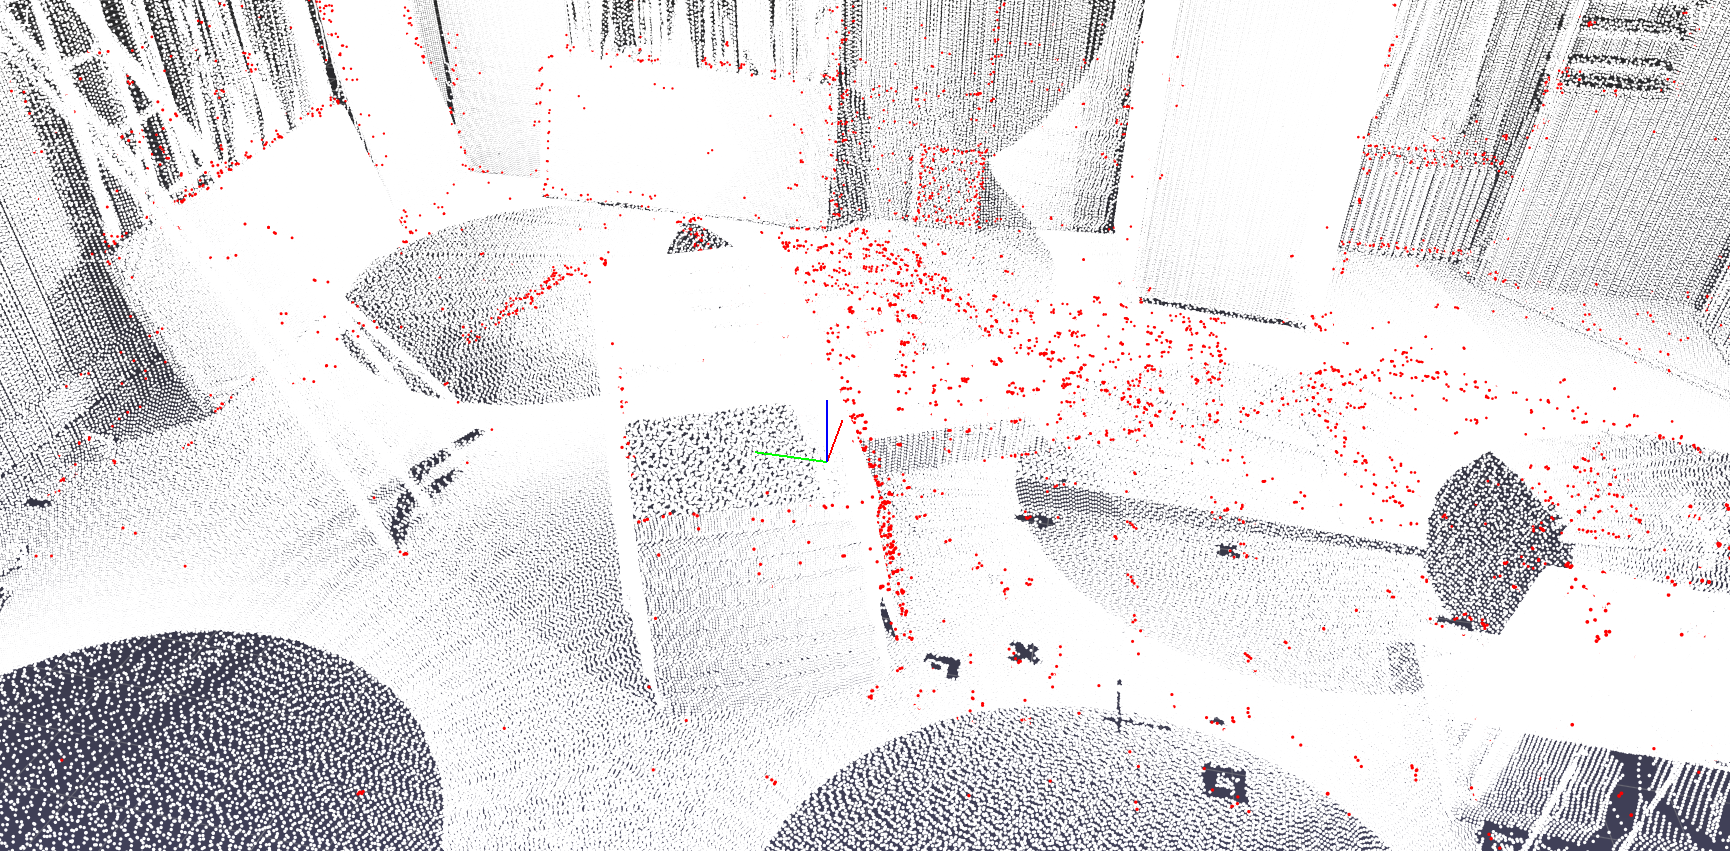
\includegraphics[width=4cm]{img/pointcloud_orb} }}%
    \qquad
    \subfloat[\centering DSM]{{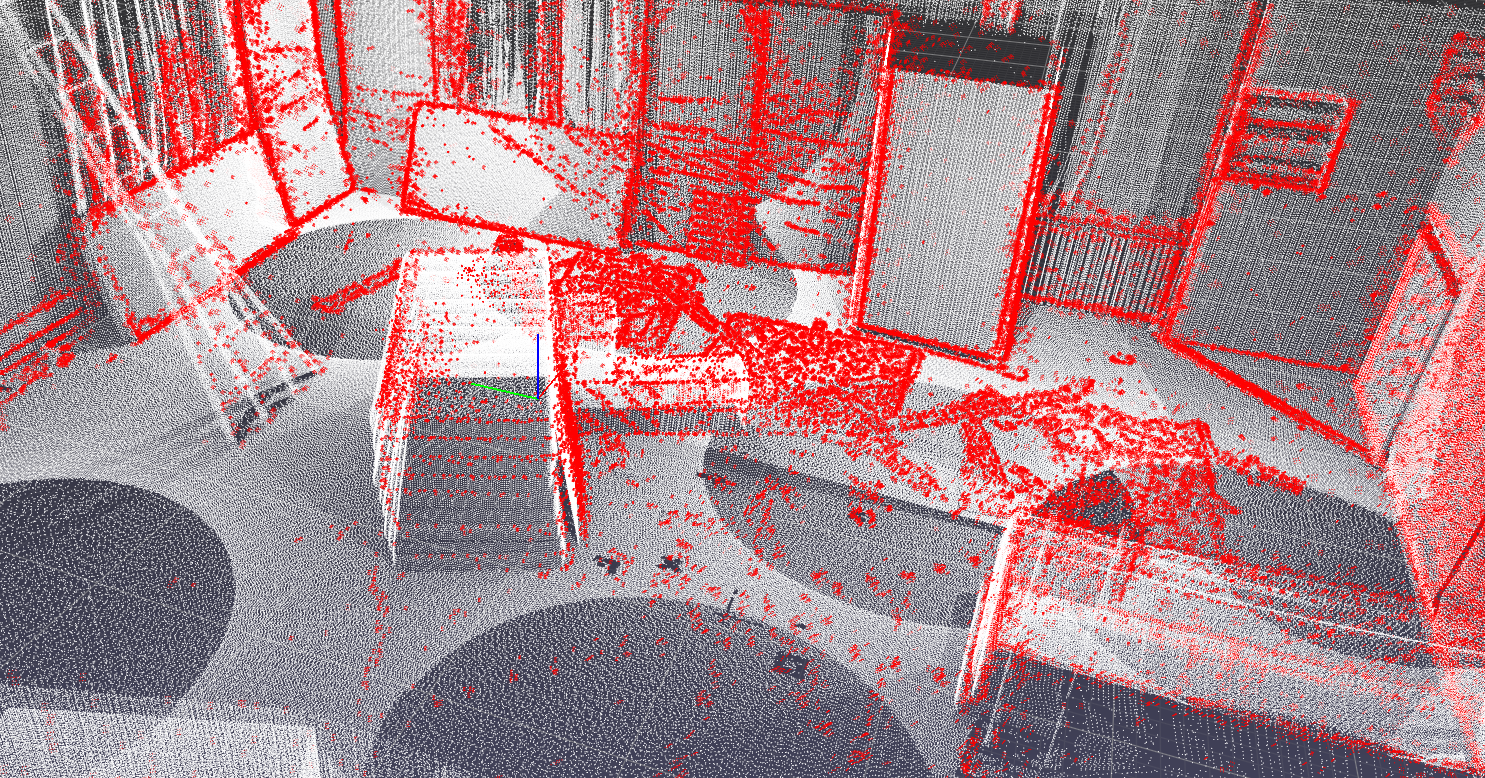
\includegraphics[width=4cm]{img/pointcloud_dsm} }}%
	\qquad
    \subfloat[\centering DSO]{{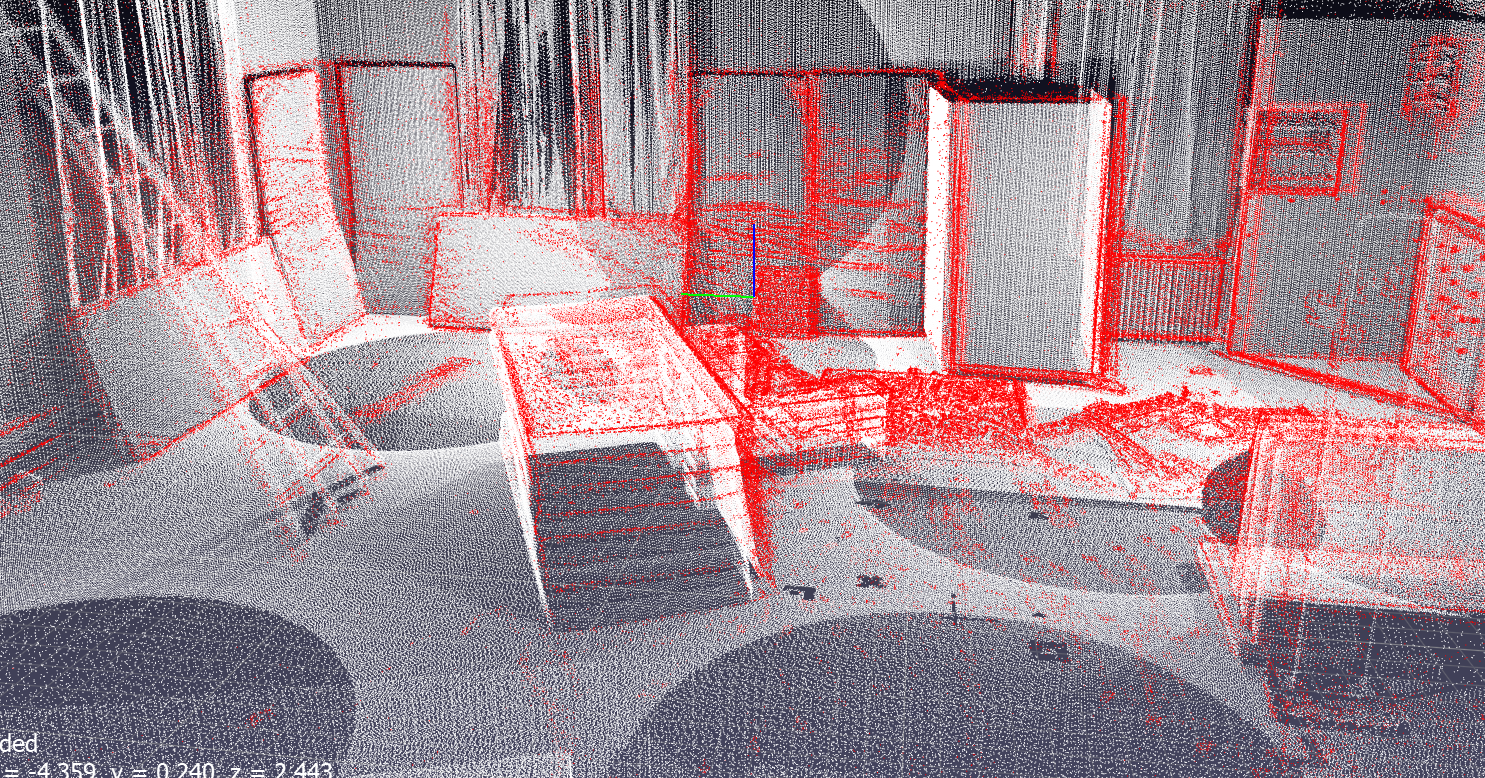
\includegraphics[width=4cm]{img/pointcloud_dso} }}%
    \caption{The groundtruth of the Pointcloud from Sequence V101 (white points) and the evaluated points by each algorithm (red points). 
	The points in Figure (a) are four times as large for better visability (ORB-SLAM generates only few points). 
	}%
    \label{fig:example}%
	\end{figure}

\section{Calculation Time}


    \chapter{Discussion}

\section{Conclusion of SLAM-Algorithm Evaluation}

% hier auch noch CNN slam erwähnen

	\begin{figure}%
    \centering
    \subfloat[\centering trajectory error]{{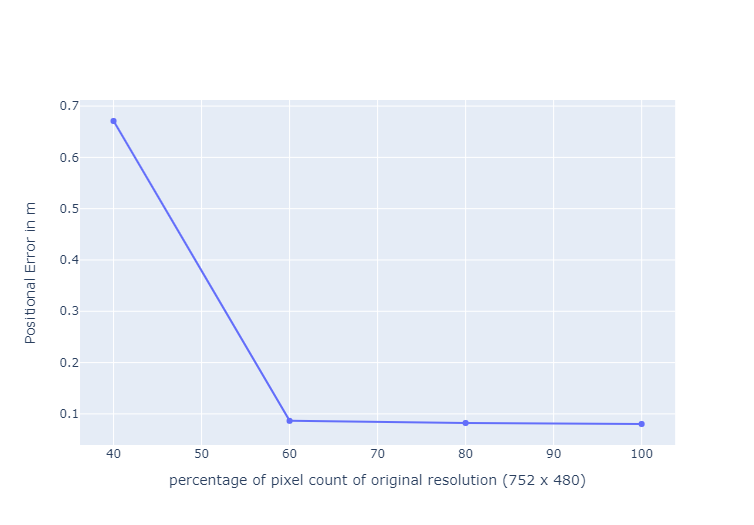
\includegraphics[width=6cm]{img/down_error.png} }}%
	\qquad
    \subfloat[\centering computation time]{{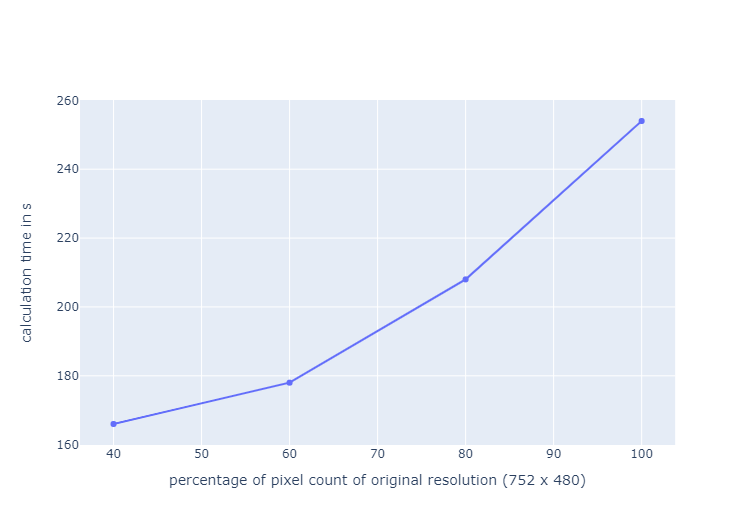
\includegraphics[width=6cm]{img/down_comp.png} }}%
    \caption{
	Influence of downsizing of the images on the trajectory error (a) and the computation time (b) for the sequence V101. 
	}%
    \label{fig:resolution}%
	\end{figure}

\section{Handlungsempfehlung}

\subsection{Framework for Trajectory Automatation}

\subsection{Trajectory Automatation using Reinforement Learning}


	

    % This places the bibliography. You can add more
    % bibliographic items it the bibliography.bib file. 
    % We suggest using a reference manager (e.g., Jabref)
    % to maintain this file
	\bibliographystyle{abbrv}
    \bibliography{bibliography}

    \newpage
    
    \backmatter

    \begin{appendices}

        % This is the actual appendix. The files referenced here
        % are just examples. You can add additional appendices
        % if necessary

    \end{appendices}

\end{document}
